\chapter{Specification and Needs Analysis}
\label{chap:Chapter 2 title}
\section{Introduction}


The success of a project heavily relies on the quality of its initiation. Therefore, the functional study phase is crucial for a successful start to the project. This chapter encompasses requirement specifications, including needs analysis involving stakeholder identification, system use cases, and the textual scenarios associated with these use cases.

\pagebreak

\section{Study of the Current State}

Orange Business Services Morocco has embraced an approach known as CI/CD to efficiently manage the development and delivery of its projects. They utilize the GitLab platform, which facilitates swift creation, compilation, testing, delivery, and deployment of software.

In their existing solution, they have established continuous integration and delivery pipelines using GitLab CI, Nexus, Docker, and Kubernetes. Here's how it operates:

\begin{itemize}
  \item Code management and updates are performed using GitLab. Developers push their code changes to the GitLab repository.
  \item The application is containerized using Docker, a technology enabling the creation of isolated and portable environments for applications.
  \item The GitLab Runner conducts a check to ensure the YAML code is correct and clean. Then, it triggers pipeline steps such as Docker image generation and their submission to the Nexus repository.
  \item Kubernetes, aided by Helm (a package manager for Kubernetes), handles the application deployment across various environments. It follows a "Push" deployment model.
\end{itemize}

This approach enables Orange Business Services Morocco to efficiently manage the development and delivery of their projects by automating processes using GitLab, Docker, Nexus, and Kubernetes. It empowers them to deliver high-quality software more rapidly.

\newpage
\section{Analysis and criticism of the current state}

While utilizing GitLab accelerates software development and deployment, there's a clear need for enhancements focused on sustainability and reducing environmental impact. An exhaustive study of the existing system was conducted to refine our project's scope and expected functionalities, aiming for a more reliable system than the previous one. Identified areas for improvement include

\begin{itemize}
  \item The current CI/CD approach relies heavily on resource-intensive technologies like Docker and Kubernetes, which contribute to increased energy consumption and carbon emissions.
  \item While effective for streamlining development workflows, the pipelines lack mechanisms for tracking and optimizing energy usage.
  \item Without visibility into the energy consumption and carbon footprint of the Kubernetes cluster, targeted strategies for reducing environmental impact are challenging to implement.
\end{itemize}

\subsection{Functional needs}
Functional requirements gathering is a crucial step in the project. This stage produces the functional specifications document, during which the expected functionalities are formalized along with all governing management rules. To address the issues identified in the existing study, the principle is to integrate monitoring tools such as Kepler (Kubernetes-based Efficient Power Level Exporter), Prometheus, and Grafana into the CI/CD pipeline. This integration aims to measure the energy consumption and CO$_2$ emissions of Orange's Kubernetes cluster, providing valuable insights for optimizing Green IT practices within the DevOps workflow.

\subsection{Non-Functional needs}

Non-functional requirements play a crucial role in system design,
because they define the attributes, constraints and restrictions to be taken into account.

These requirements, also called system qualities, guarantee the
user-friendliness and overall efficiency of the system. If any of these requirements are not met,
the system risks not meeting the internal needs of the company, users
or the market.

\begin{itemize}
  \item \textbf{Accuracy}: The system must provide accurate measurements of energy consumption and CO$_2$ emissions to support informed decision-making.
  \item \textbf{Scalability}: Ensure scalability to handle increasing data volumes as the size of the Kubernetes cluster grows.
  \item \textbf{Reliability}: The solution should be reliable, with minimal downtime, to maintain continuous monitoring and data collection.
  \item \textbf{Security}: Implement robust security measures to safeguard sensitive energy consumption and emission data from unauthorized access or tampering.
  \item \textbf{Performance}: Ensure efficient performance to deliver timely insights and visualizations, even during peak usage periods.
  \item \textbf{Ease of Use}: Design an intuitive user interface that allows administrators to easily configure monitoring settings and interpret data visualizations.
  \item \textbf{Compatibility}: Ensure compatibility with existing infrastructure and tools used within Orange Business Services Morocco, such as Prometheus, Grafana, and Kepler.
\end{itemize}


\section{DevOps appraoch}
The word DevOps is a combination of the terms development and operations, meant to represent a collaborative or shared approach to the tasks performed by a company's application development and IT operations teams.
The DevOps methodology aims to shorten the systems development lifecycle and provide continuous delivery with high software quality. These characteristics help ensure a culture of building, testing, and releasing software that is more reliable and at a high velocity.

\section{Definition of CI/CD}
\textit{Continuous Integration (CI)} is a software development practice where developers frequently merge their code changes into a central repository, typically multiple times a day. Each merge triggers an automated build and testing process. The primary goal of CI is to detect and address issues early in the development cycle, which helps in maintaining code quality and reducing integration problems. By integrating frequently, developers can identify bugs early, facilitating easier and quicker fixes.

\textit{Continuous Delivery (CD)} extends CI by automatically preparing code changes for a release to production. It ensures that the software can be reliably released at any time, with the deployment process being automated but requiring manual approval. Continuous Deployment is a further extension of CD where every change that passes all stages of the production pipeline is automatically released to customers without human intervention. This practice reduces the lead time for delivering new features and fixes, thus providing rapid feedback to developers and stakeholders.

\section{Definition of Green IT}

Green IT, also known as Green Information Technology, refers to environmentally sustainable computing practices. It encompasses a broad range of strategies aimed at minimizing the environmental impact of IT operations. This includes optimizing energy consumption, reducing electronic waste, and promoting the use of eco-friendly technologies. 

The goal of Green IT is to create more efficient and sustainable systems by implementing practices such as energy-efficient hardware, virtualization, and effective cooling systems in data centers. It also involves the adoption of cloud computing to optimize resource use and the implementation of robust recycling programs for electronic devices.

\section{Green DevOps:}
Green DevOps extends DevOps principles, focusing on resource efficiency while staying agile. It emphasizes sustainability, reducing environmental impact, and integrating eco-friendly strategies into software development. The goal is to balance technological innovation with ecological responsibility.
\begin{figure}[H]
  \centering
  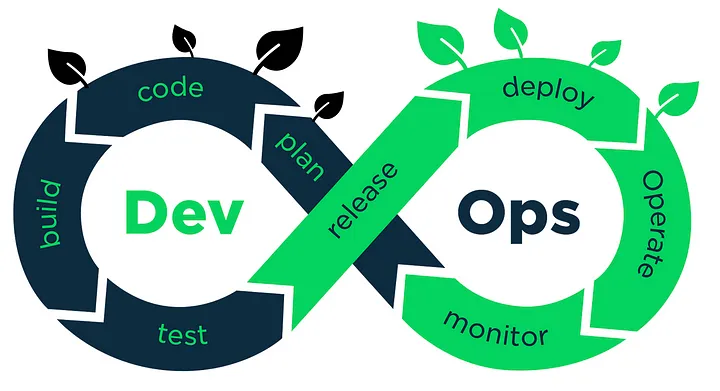
\includegraphics[width=16cm]{Figures/devgreenops.png}
  \caption{Green DevOps}
\end{figure}
\subsection{The Fundamental Principles of Green DevOps}
Green DevOps is nothing more than an extension of DevOps. It shouldn't be viewed as an upheaval of all DevOps principles. We retain all DevOps principles but adjust them as finely as possible to optimize resource usage.

Green DevOps relies on the following concepts:
\begin{itemize}
  \item \textbf{Infrastructure Optimization:} Choosing eco-friendly data centers, energy-efficient hardware, and effective resource utilization are pillars of Green DevOps. The goal is to reduce energy consumption while maintaining performance.
  
  \item \textbf{Reduction of E-waste:} This involves minimizing over-provisioning of IT resources, properly managing electronic waste, and promoting hardware component recycling.
  
  \item \textbf{Automation and Process Optimization:} Automation is at the core of DevOps, but it holds even greater importance in the context of Green DevOps. Automating tasks reduces energy consumption by minimizing unused resources and enabling fine-grained resource management.
  
  \item \textbf{Carbon Impact Assessment:} To truly become "green," measurement is necessary. Green DevOps integrates tools and metrics to continuously assess and monitor the carbon footprint of projects. This helps identify areas needing improvement and track progress.
  
  \item \textbf{Reduction of Cycle Times:} Shorter development cycles mean less energy consumption and faster time to market. By reducing delays, Green DevOps contributes to the competitiveness of the business while minimizing its environmental impact.
  
  \item \textbf{Awareness:} DevOps teams need to be aware of environmental issues. Employee training and engagement are essential to fostering the adoption of sustainable practices.
\end{itemize}

\subsection{The Benefits of Green DevOps}

\begin{itemize}
  \item \textbf{Cost Reduction}: Less wasted resources, time saved, and efficient resource utilization result in a significant reduction in operating and infrastructure costs.
  
  \item \textbf{Quality Improvement}: Green DevOps practices encourage automation, monitoring, and rigorous testing, leading to better software quality, fewer bugs, and an enhanced user experience.
  
  \item \textbf{Social Responsibility}: Companies adopting Green DevOps demonstrate their commitment to environmental sustainability, which can enhance their brand image and attract new customers and talents.
  
  \item \textbf{Regulatory Compliance}: With an increasing number of environmental regulations in place, Green DevOps helps companies comply with standards and avoid potential penalties.
\end{itemize}

\section{DevOps Monitoring}
DevOps monitoring is the process of tracking and measuring the performance of applications and systems in order to help software development teams identify and resolve potential issues more quickly. This is typically done via a manual or automated DevOps monitoring solution or a collection of continuous monitoring tools that gather data

\subsection{DevOps Monitoring Use Cases}

The main benefit of DevOps monitoring is its ability to define, track, and measure KPIs across all aspects of DevOps. Here are some specific use cases of DevOps monitoring:

\begin{itemize}
  \item \textbf{Detect and Report Errors Earlier:}
  Flagging issues to DevOps teams more quickly means they can resolve them before they impact user experience. Early detection and reporting of errors allow for prompt resolution, minimizing disruptions and maintaining a smooth user experience.
  \item \textbf{Reduce System Downtime:}
  DevOps monitoring tools provide continuous oversight of databases, applications, and networks, enabling teams to resolve issues before system downtimes occur. By proactively identifying potential problems, teams can take preemptive actions to avoid outages and ensure system reliability.
  \item \textbf{Enhance Observability of DevOps Components:}
  Easily identify when various systems and applications in your DevOps stack degrade in performance, cost, security, or other factors to avoid problems down the road. Enhanced observability enables teams to maintain optimal performance and security by monitoring and analyzing system behavior continuously.

  \item \textbf{Uncover Root Cause of Issues Faster:}
  Continuous tracking of logs and metrics helps teams identify the root cause — where a problem started or occurred. This allows engineers to detect patterns in system behavior to anticipate and prevent future issues, improving mean time to detection (MTTD), mean time to repair (MTTR), and mean time to isolate (MTTI).
\end{itemize}

\section{Needs Analysis}
\label{sec:needs_analysis}

After identifying the functional and non-functional requirements of the project, it is essential to clearly define the stakeholders of the system and the different use cases. This step is crucial for preparing the design phase of the project.

\subsection{Identification of Stakeholders}
\label{subsec:identification_stakeholders}

Identifying stakeholders is a fundamental step in any development project. It helps to understand the interactions and measure the influence of each group on the actions to be undertaken. But what exactly is a stakeholder? A stakeholder can be a physical person or a legal entity that participates in or is affected by the action or project in question. It is important to clearly specify the action or series of actions for which we seek to determine who the stakeholders are and what they represent.

In the context of integrating Green IT into DevOps practices at Orange Business Services Morocco, we identify the following stakeholders:

\begin{itemize}
  \item \textbf{Platform Admin Team}: Responsible for setting up staging and production environments, managing cluster extension modules, and other cluster resources (controllers and admission webhooks), integrating development team repositories using customized GitRepository resources, and configuring how development team repositories are reconciled on each cluster.
  
  \item \textbf{Development Team}: Configures application definitions at the Kubernetes deployment level, manages Helm releases, configures how applications are reconciled across environments, and oversees the promotion of applications between environments.
  
  \item \textbf{Green IT Team}: Responsible for analyzing the energy consumption and CO$_2$ emissions of the Kubernetes clusters. 
  
  \item \textbf{GitLab}: A secondary stakeholder that manages team access and coordinates the CI/CD processes.
\end{itemize}

By identifying these stakeholders and their respective roles, we can ensure a comprehensive approach to integrating Green IT into our DevOps practices, balancing rapid software delivery with environmental responsibility.

\subsection{Use Case Diagrams}
\label{subsec:use_case_diagrams}

The role of use case diagrams in UML is to model the behavior of a system and capture the associated requirements. These diagrams highlight the high-level functions of the system and define its scope. They also help identify the interactions between the system and its stakeholders. However, it is important to note that use case diagrams focus on what the system does and how the stakeholders use it, without delving into its internal workings.

In this perspective, a use case represents a function that the system performs to achieve a specific goal for the user. It should generate an observable result that holds value for the system's user. On the other hand, a stakeholder represents the role of a user who interacts with the modeled system. This could be a human, an organization, a machine, or another external system.

The relationships between elements in use case diagrams play a crucial role. As UML model elements, these relationships establish semantic links that define the structure and behavior among different elements of the model.

In the context of integrating Green IT into DevOps at Orange Business Services Morocco, we present the global use case diagram of our solution in Fig. \ref{fig:use_case_diagram}. This diagram provides an overview of the interactions between the stakeholders and the various functionalities of the system.




\section{}



















